\documentclass{article}
\usepackage[left=3cm,right=3cm,top=2cm,bottom=2cm]{geometry}
\usepackage[ngerman]{babel}
\usepackage{amsmath}
\usepackage{amssymb}
\usepackage{amsthm}
\usepackage{hyperref}

\usepackage{graphicx}
\usepackage{subfig}

\setlength{\parindent}{0mm}

\newcommand{\R}[0]{\mathbb{R}}
\newcommand{\N}[0]{\mathbb{N}}
\newcommand{\F}[0]{\mathcal{F}}
\newcommand{\E}[0]{\mathbb{E}}
\newcommand{\Ssp}[0]{\mathcal{S}}
\newcommand{\C}[0]{C^{\infty}_0}

\DeclareRobustCommand{\loongrightarrow}{%
  \DOTSB\relbar\joinrel\relbar\joinrel\rightarrow
}

\title{Applied Problems in Data Science}
\author{Yannik Höll}
\date{\today}

\theoremstyle{plain}
\newtheorem{thm}{Satz}[section]

\theoremstyle{definition}
\newtheorem{defin}[thm]{Definition}
\newtheorem{bem}[thm]{Bemerkung}
\newtheorem{lemma}[thm]{Lemma}
\newtheorem{definthm}[thm]{Definition \& Satz}

\DeclareMathOperator{\esssup}{esssup}

\begin{document}

\nocite{*}

\maketitle

\section{Inverse Faltung}

\subsection{Klassische Fouriertransformation und Faltung}

Für folgende Definitionen sei $n \in \mathbb{N} \setminus \{ 0 \}$.

\begin{defin}
    Seien $f,g \in L^1(\R^n)$. \\
    Dann ist die \textbf{Faltung} von $f$ mit $g$ für $x \in \R^n$ definiert als:
    \begin{equation}
        (f \star g)(x) := \int_{\R^n} f(x - y) g(y) dy
    \end{equation}
\end{defin}

\begin{thm}\label{thm:konvmap}
    Die Faltung $\_ \star \_$ ist eine wohldefinierte Abbildung von $L^1(\R^n) \times L^1(\R^n)$ nach $L^1(\R^n)$.
\end{thm}

\begin{proof}
    Seien $f,g \in L^1(\R^n)$ und sei $F: \R^n \times \R^n \to \R, (x,y) \mapsto f(x - y)g(y)$. Die Funktion $F$ ist messbar,
    weil $g$ messbar ist und weil $\tilde{f} = f \circ \tau_{-y}$ mit $\tau_y: \R^n \to \R, x \mapsto x + y$ eine Komposition messbarer Funktionen ist
    und somit messbar. Ferner gilt $F = \tilde{f}g$ und damit ist $F$ das Produkt messbarer Funktionen.

    Nun kann man schließen:
    \begin{align*}
        \hspace{-23px}\int_{\R^n \times \R^n} \left| F(x,y)\right| d(x,y) &\overset{(*)}{=} \int_{\R^n}\int_{\R^n} \left| F(x,y)\right| dxdy \\
        &= \int_{\R^n}\int_{\R^n} \left|f(x - y)g(y)\right| dxdy \\
        &= \int_{\R^n}\int_{\R^n} \left| f(x - y) \right| \left| g(y) \right| dx dy \\
        &= \int_{\R^n} \underbrace{\left(\int_{\R^n} \left| f(x - y) \right| dx \right)}_{=\lVert f \rVert_1} \left| g(y) \right| dy \\
        &= \lVert f \rVert_1 \left(\int_{\R^n} \left| g(x) \right| dx\right) \\ 
        &= \lVert f \rVert_1 \lVert g \rVert_1 < \infty
    \end{align*}
    Die Gleicheit $(*)$ folgt aus dem Satz von Fubini-Tonelli, weil $F$ messbar ist.

    Somit ist $F \in L^1(\R^n \times \R^n)$.
    
    Aus dem Satz von Fubini folgt, dass die Abbildung $x \mapsto \int_{\R^n} F(x,y) dy = (f\star g)(x)$ im $L^1(\R^n)$ liegt.
\end{proof}

\begin{lemma}\label{lem:convsym}
    Für $f,g \in L^1(\R^n)$ gilt: $f \star g = g \star f$.
\end{lemma}

\begin{proof}
    Seien $f,g \in L^1(\R)$ und $x \in \R$, dann folgt:
    \begin{align*}
        (f \star g)(x) &= \int_{-\infty}^{\infty} f(x - y) g(y) dy \\
        &= \int_{\infty}^{-\infty} f(\tilde{y}) g(x - \tilde{y}) (-1)d\tilde{y}, \hspace{20px} \tilde{y} = x - y \\
        &= \int_{-\infty}^{\infty} f(\tilde{y}) g(x - \tilde{y}) d\tilde{y} \\
        &= (g \star f)(x)
    \end{align*}
    Somit gilt die Kommutativität der Faltung für den Fall $n=1$. Die Kommutativität für alle $n$ folgt nun aus Satz \ref{thm:konvmap}, da nämlich
    $f \star g \in L^1(\R)$ gilt:
    \begin{equation*}
        (f \star g)(x) = \int_{\R^n} f(x - y)g(y) dy = \int_{-\infty}^{\infty} \int_{-\infty}^{\infty} \cdots \int_{-\infty}^{\infty} f(x_1 - y_1, x_2 - y_2, \cdots, x_n - y_n) g(y_1, y_2, \cdots, y_n) dy_1 dy_2 \cdots dy_n
    \end{equation*}
    und man kann die Substitution wie oben auf jede Diemension einzeln anwenden.
\end{proof}

\begin{defin} Die \textbf{Fourier-Transformation} einer Funktion $f \in L^1(\R^n)$ ist definiert durch:
    \begin{equation}
        (\mathcal{F}f)(\xi) := \int_{\R^n} f(x) \cdot e^{-2\pi i x \cdot \xi} dx
    \end{equation}
    für $x, \xi \in \R^n$. Dabei ist $x \cdot \xi$ das Skalarprodukt im $\R^n$.
\end{defin}

\begin{thm}\label{thm:ft-map}
    Die Fouriertransformation ist eine wohldefinierte Abbildung von $L^1(\R^n) \to L^{\infty}(\R^n)$.
\end{thm}

\begin{proof}
    Sei $f \in L^1(\R^n)$, dann gilt:
    \begin{align*}
        \forall \xi \in \R^n: |\mathcal{F}f(\xi)| &= \Bigg\lvert \int_{\R^n} f(x) \cdot e^{-2\pi i x \cdot \xi} dx \Bigg\rvert \\
        &\leq \int_{\R^n} \lvert f(x) \rvert \lvert e^{-2\pi i x \cdot \xi} \rvert dx \\
        &= \int_{\R^n} \lvert f(x) \rvert dx \\
        &= \lVert f \rVert_{L^1(\R^n)} < \infty
    \end{align*}
    Daraus folgt nun: $\lVert\mathcal{F}f\rVert_{\infty} = \esssup\limits_{\xi \in \R^n} |\mathcal{F}f(\xi)| \leq \lVert f \rVert_{L^1(\R^n)} < \infty$
\end{proof}

\begin{defin}
    Die \textbf{Inverse Fouriertransformation} einer Funktion $f \in L^1(\R^n)$ ist definiert durch:
    \begin{equation}
        (\mathcal{F}^{-1}f)(\xi) := \int_{\R^n} f(x) \cdot e^{2\pi i x \cdot \xi} dx
    \end{equation}
    für $x, \xi \in \R^n$. Dabei ist $x \cdot \xi$ das Skalarprodukt im $\R^n$.
\end{defin}
Der Nachweis der Wohldefiniertheit funktioniert genauso, wie bei der Fouriertransformation.

\begin{lemma}\label{lem:l1linfty}
    Seien $f\in L^1(\R^n), g \in L^{\infty}(\R^n)$, dann gilt: $f \cdot g \in L^1(\R^n)$.
\end{lemma}

\begin{proof}
    \begin{align*}
        \lVert f \cdot g \rVert_1 &= \int_{\R^n} |f(x)g(x)| dx \\
        &\leq \int_{\R^n} |f(x)| \lVert g(x) \rVert_{\infty} dx \\
        &= \lVert g(x) \rVert_{\infty} \int_{\R^n} |f(x)| dx \\
        &= \lVert g(x) \rVert_{\infty} \lVert f(x) \rVert_1 < \infty
    \end{align*}
\end{proof}

\begin{thm}\label{thm:convinvl1}
    \textbf{Faltungssatz im $L^1(\R^n)$} \\
    Seien $f,g \in L^1(\R^n)$ und $\mathcal{F}g \in L^1(\R^n)$. Dann gilt:
    \begin{equation}
        \mathcal{F}(f \star g) = \mathcal{F}f \cdot \mathcal{F}g
    \end{equation}

    \begin{proof} \cite[S. 371f.]{howell2016principles}
        Der Beweis ist abgeschlossen, wenn gezeigt wurde, dass $\F^{-1} (\F f \cdot \F g) = f \star g$. 
        
        Sei $F(\omega) := \F f(\omega)$ und $G(\omega) := \F g(\omega)$. Als erstes ist festzustellen, dass $\F^{-1} (F(\omega) G(\omega))$ existiert, weil
        $G \in L^1(\R^n)$ ist und nach Lemma \ref{lem:l1linfty} somit $F \cdot G \in L^1(\R^n)$ ist. Es folgt: \\
        \begin{align*}
            \F^{-1} (F(\omega) G(\omega)) &= \int_{\R^n} F(\omega) G(\omega) \cdot e^{2\pi i \omega \cdot t} d\omega \\
            &= \int_{\R^n} \Bigg\lbrack \int_{\R^n} f(s) \cdot e^{-2\pi i s \cdot \omega} ds \Bigg\rbrack G(\omega) \cdot e^{2\pi i \omega \cdot t} d\omega \\
            &= \int_{\R^n} \int_{\R^n} f(s) G(\omega) \cdot e^{2\pi i \omega \cdot (s - t)} ds d\omega
        \end{align*}
        Seien $s,t \in \R^n$, dann gilt:
        \begin{equation*}
            \forall \xi \in \R^n: |e^{2\pi i \omega \cdot (s - t)}| = 1 \Rightarrow \esssup\limits_{\omega \in \R^n} |e^{2\pi i \omega \cdot (s - t)}| = 1 < \infty
        \end{equation*}
        Und somit ist $e^{2\pi i \omega \cdot (s - t)} \in L^{\infty}(\R^n)$ bezüglich $\omega$ und aus mit einem ähnlichen Argument auch bezüglich $s$.
        Daraus und aus Lemma \ref{lem:l1linfty} folgt, dass $f(s) G(\omega) \cdot e^{2\pi i \omega \cdot (s - t)} \in L^1(\R^n \times \R^n)$ bezüglich $\omega$ und $s$ ist.
        Somit sind die Vorraussetzungen des Satzes von Fubini erfüllt und man kann die Integrationsreihenfolge vertauschen:
        \begin{align*}
            \F^{-1} (F(\omega) G(\omega)) &= \int_{\R^n} \int_{\R^n} f(s) G(\omega) \cdot e^{2\pi i \omega \cdot (s - t)} d\omega ds \\
            &= \int_{\R^n} f(s) \Bigg \lbrack \int_{\R^n} G(\omega) \cdot e^{2\pi i \omega \cdot (t - s)} d\omega \Bigg \rbrack ds \\
            &\overset{*}{=} \int_{\R^n} f(s) g(t-s) ds = g \star f \overset{\text{Lemma \ref{lem:convsym}}}{=} f \star g
        \end{align*}
        Die Gleichheit $(*)$ folgt aus der Tatsache, dass sowohl $g(x)$ als auch $G(\omega)$ im $L^1(\R^n)$ liegen.
    \end{proof}
\end{thm}

Man kann an der zusätzlich benötigten Bediengung $\mathcal{F}g \in L^1(\R^n)$ im Faltungssatz erkennen, dass der $L^1(\R^n)$ nicht der natürlichste Raum ist, um die Fouriertransformation zu definieren.
Deswegen wird im folgenden die Definition auf einem alternativem Raum vorgenommen, auf dem die Transformation bessere Eigenschaften hat.

\subsection{Umkehrformel im $L^2$}

\begin{defin}
    Eine Funktion $f \in C^{\infty}$ heißt \textbf{schnell fallend}, wenn $\forall \alpha \in \N^n: \lim\limits_{|x| \to \infty} x^{\alpha}f(x) = 0$.

    Der \textbf{Schwartz-Raum} ist wie folgt definiert:
    \begin{equation*}
        \Ssp(\R^n) := \{ f \in C^{\infty}(\R^n) \: | \: \forall \alpha,\beta \in \N^n: \sup\limits_{x \in \R^n} \left| x^\alpha\partial_{\beta}f(x) \right| < \infty \}
    \end{equation*}
\end{defin}
Anders formuliert sind Schwartz-Funktionen beliebig oft differenzierbare schnell fallende Funktionen, bei denen jede Ableitung ebenfalls eine schnell fallende Funktion ist.

\begin{bem}\label{bem:C0sub}
    $C^{\infty}_0(\R^n) \subseteq \Ssp(\R^n)$
\end{bem}

\begin{proof}
    Sei $f \in \C(\R^n)$. Da $f$ stetig ist und ein kompakten Träger besitzt folgt: $\sup\limits_{x \in \R^n} |f(x)| < \infty$.

    Für $\forall \beta \in \N^n: \partial_x^{\beta} f \in \C(\R^n) \Rightarrow \sup\limits_{x \in \R^n} |\partial_x^{\beta}f(x)| < \infty$.

    Sei $\alpha \in \N^n$. Sei ${\rm supp} f$ der Träger von $f$ und wähle $a \in \R_{\geq 0}$, sodass ${\rm supp}f \subseteq [-a, a]$, dann gilt für $\forall x \notin [-a, a]$:
    \begin{equation}
        x^{\alpha}f(x) = 0
    \end{equation}

    Und da $x \mapsto x^{\alpha} \in C^{\infty}(\R^n)$ gilt $x \mapsto x^{\alpha}f(x) \in \C(\R^n)$ für $\forall \alpha \in \N^n$.
    
    Daraus kann man nun schließen, dass $\forall \alpha, \beta \in \N^n: \sup\limits_{x \in \R^n} |x^{\alpha}\partial_x^{\beta}f(x)| < \infty$.
\end{proof}

\begin{lemma}\label{lem:C0dense}
    $\C(\R^n)$ liegt dicht im Raum $L^2(\R^n)$.
\end{lemma}

\begin{proof}
    Siehe \cite[S. 115, Satz 2.15(3)]{alt2016linear}.
\end{proof}

\begin{lemma}\label{lem:slp}
    $\forall 1 \leq p < \infty: \Ssp(\R^n) \subseteq L^p(\R^n)$
\end{lemma}

\begin{proof}\cite[S. 230f.]{werner2006funktionalanalysis}
    Sei $f \in \Ssp(\R^n)$ und $1 \leq p < \infty$. Es gilt die Abschätzung:
    \begin{equation}
        \forall x\in \R^n, m\in \N\exists c>0: |f(x)|^p \leq \left(\frac{c}{1 + |x|^m}\right)^p
    \end{equation}

    Dann folgt für $pm - (n-1) > 1$:
    \begin{align*}
        \int_{\R^n} |f(x)|^p dx &\leq \int_{\R^n} \left(\frac{c}{1 + |x|^m}\right)^p dx \\
        &= c^p \omega_{n - 1} \int_{0}^{\infty} \left(\frac{1}{1 + r^m}\right)^pr^{n - 1}dr \\
        &= c^p \omega_{n - 1} \int_{0}^{\infty} \underbrace{\left(\frac{r^{\frac{n-1}{p}}}{1 + r^m}\right)^p}_{\sim o(\frac{1}{1+r})} dr < \infty
    \end{align*}
    wobei $\omega_{n-1}$ der Oberflächeninhalt der $n$-Späre ist.
\end{proof}

\begin{defin}
    Die \textbf{Fouriertransformation} auf dem Schwartz-Raum ist für $f \in \Ssp(\R^n), \xi \in \R^n$ definiert durch:
    \begin{equation}
        \F f(\xi) := \int_{\R^n} f(x) \exp^{-2\pi i x \cdot \xi} dx
    \end{equation}
    Dabei ist $x \cdot \xi$ wieder das Skalarprodukt im $\R^n$.
    Die inverse Transformation wird auch analog wie bei $L^1(\R^n)$ definiert.
\end{defin}

\begin{thm}
    Die Fouriertransformation ist eine stetige Abbildung von $\Ssp(\R^n)$ nach $\Ssp(\R^n)$.
\end{thm}

\begin{proof}\cite[S. 424, Theorem 24.1.1]{ebert2018methods}
    Sei $f \in \Ssp(\R^n)$ und $\alpha, \beta \in \N^n$. Dann gilt:
    \begin{align*}
        \xi^{\beta}\partial_{\xi}^{\alpha}\F f(\xi) &= \int_{\R^n} (-2\pi i x)^{\alpha} \xi^{\beta} f(x) e^{-2\pi i x \cdot \xi} dx \\
        &= (2\pi)^{|\alpha| - |\beta|} \int_{\R^n} i^{|\beta|} \partial_{x}^{\beta}(e^{-2\pi i x \cdot \xi}) (-ix)^{\alpha} f(x) dx \\
        &\overset{\text{*}}{=}i^{|\beta|}(2\pi)^{|\alpha| - |\beta|} \int_{\R^n} e^{-2\pi i x \cdot \xi} \partial_{x}^{\beta}((-ix)^{\alpha}f(x)) dx \\
        &= i^{|\beta|}(2\pi)^{|\alpha| - |\beta|} \int_{\R^n} e^{-2\pi i x \cdot \xi} (1+|x|^2)^{-\frac{n+1}{2}} (1+|x|^2)^{\frac{n+1}{2}} \partial_{x}^{\beta}((-ix)^{\alpha}f(x)) dx
    \end{align*}
    Die Gleichheit bei $(*)$ kommt durch die Partielle Integration, wobei $\partial_{x}^{\beta}(e^{-2\pi i x \cdot \xi})$ integriert wird und $(-ix)^{\alpha} f(x)$ differenziert wird. Die entstehenden Randterme veschwinden, weil $f, x \mapsto e^{-2\pi i x\cdot \xi} \in \Ssp(\R^n)$.
    
    Setze nun $C := i^{|\beta|}(2\pi)^{|\alpha| - |\beta|} \sup\limits_{x \in \R^n} |(1+|x|)^{\frac{n+1}{2}} \partial_{x}^{\beta}((-ix)^{\alpha}f(x))|$. 
    
    Das Supremum existiert, da $f \in \Ssp(\R^n)$. Es gilt die Abschätzung:
    
    \begin{equation*}
        |\xi^{\beta}\partial_{\xi}^{\alpha}\F f(\xi)| \leq C \int_{\R^n} (1+|x|^2)^{-\frac{n+1}{2}} dx < \infty
    \end{equation*}

    Daher folgt, dass $\forall \alpha, \beta\in \N^n: \sup\limits_{\xi \in \R^n} \left|\xi^{\beta}\partial_{\xi}^{\alpha}\F f(\xi)\right| < \infty \Rightarrow \F f \in \Ssp(\R^n)$

    Sei nun $\{f_k\}_{k\in\N} \subseteq \Ssp(\R^n)$ eine Folge von Schwartz-Funktionen, die gegen einen Grenzwert $f \in \Ssp(\R^n)$ konvergiert, 
    d.h. $\forall \alpha,\beta\in\N^n: \sup\limits_{x \in \R^n} |x^{\alpha}\partial_x^{\beta}(f_k - f)| \overset{k \to \infty}{\loongrightarrow} 0$.
    Mit der gleichen Abschätzung nun für $f_k - f$ erhält man auch $\forall \alpha,\beta\in\N^n: \sup\limits_{x \in \R^n} |x^{\alpha}\partial_x^{\beta}(\F f_k - \F f)| \overset{k \to \infty}{\loongrightarrow} 0$.
    Daraus folgt die Stetigkeit der Abbildung.
\end{proof}

\begin{thm}
    Die Fouriersche Umkehrformel gilt in $\Ssp(\R^n)$, d.h.: $\forall f\in \Ssp(\R^n): (\F^{-1} \circ \F)(f) = f$.
\end{thm}

\begin{proof}\cite[S. 424, Theorem 24.1.1]{ebert2018methods}
    Sei $g \in C^{\infty}_0(\R^n)$ und für $\varepsilon > 0$ definiere $g_{\varepsilon} := \varepsilon^{-n} g(\frac{1}{\varepsilon})$.

    Dann gilt für $f \in \Ssp(\R^n), x \in \R^n$:
    \begin{equation}\label{eq:mol}
        \lim\limits_{\varepsilon \to 0} \lVert (g_{\varepsilon} \star f) - f\rVert_2 = 0
    \end{equation}
    Zusätzlich gilt $g_{\varepsilon} \star f \in C^{\infty}(\R^n)$.
    Ein Beweis der Gleichung \ref{eq:mol} befindet sich in \cite[S. 183ff.]{walter1966analysis}.

    Sei nun $f \in \Ssp(\R^n)$ und sei $\chi(x) = \begin{cases}
        1, |x| \leq 1, \\
        0, |x| \geq 2
    \end{cases}$ mit $\chi \in C^{\infty}_0(\R^n)$ also mit einem glatten Übergang im Intervall $(1, 2)$.

    Es folgt:
    \begin{align*}
        (\F^{-1} \circ \F)(f)(x) &= \int_{\R^n} \int_{\R^n} e^{-2\pi (x - y) \cdot \xi} f(y) dy d\xi \\
        &= \lim\limits_{\varepsilon \to 0} \int_{\R^n} \int_{\R^n} e^{-2\pi (x - y) \cdot \xi} f(y) \chi(\varepsilon \xi) dy d\xi \\
        &= \lim\limits_{\varepsilon \to 0} \int_{\R^n} \int_{\R^n} f(y) \varepsilon^{-n} e^{-2 \pi \frac{x - y}{\varepsilon} \cdot z}\chi(z) dy dz, \hspace*{20px} z = \varepsilon \xi \\
        &\overset{*}{=} \lim\limits_{\varepsilon \to 0} \int_{\R^n} f(y) \varepsilon^{-n} \int_{\R^n} e^{-2 \pi \frac{x - y}{\varepsilon} \cdot z}\chi(z) dz dy\\
        &= \lim\limits_{\varepsilon \to 0} (f \star g_{\varepsilon})(x) \hspace*{20px} (\star)
    \end{align*}
    mit $g(x) = \int_{\R^n}e^{-2\pi ix \cdot z} \chi(z) dz$. Das ist eine $C^{\infty}_0(\R^n)$ Funktion, weil $z \mapsto e^{-2\pi ix \cdot z} \chi(z) \in C^{\infty}_0(\R^n)$ 
    ist das Integral die Regularität nicht verschlechtert und der kompakte Träger bleibt erhalten, weil $\chi(z) = 0, \forall z \in \R^n: |z| \geq 2$.

    Die Intergrationsreihenfolge bei $(*)$ kann vertauscht werden durch den Satz von Fubini,
    da $(y, z) \mapsto f(y) e^{-2 \pi \frac{x - y}{\varepsilon} \cdot z}\chi(z) \in L^1(\R^n \times \R^n)$, weil $e^{-2 \pi \frac{x - y}{\varepsilon} \cdot z} \in L^{\infty}(\R^n)$ und $\chi \in L^1(\R^n),f \in \Ssp(\R^n) \subseteq L^1(\R^n)$.
    
    Aus Gleichung \ref{eq:mol}, $(\star)$ und $f \star g_{\varepsilon} \in C^{\infty}(\R^n)$ folgt nun $(\F^{-1} \circ \F)(f)(x) = f(x)$.
\end{proof}

\begin{lemma}\label{lem:Ssp1}
    Seien $f,g \in \Ssp(\R^n)$:
    \begin{enumerate}
        \item $\int_{\R^n}\F^{-1}f(x)\overline{g(x)}dx = \int_{\R^n}f(\xi)\overline{\F g(\xi)} d\xi \iff (\F f, g)_2 = (f, \F^{-1}g)_2$
        \item $\int_{\R^n}\F f(x)\overline{g(x)}dx = \int_{\R^n}f(\xi)\overline{\F^{-1} g(\xi)} d\xi \iff (\F^{-1} f, g)_2 = (f, \F g)_2$
    \end{enumerate}
\end{lemma}

\begin{proof}\cite[S. 427f.]{ebert2018methods}
    
    Beweis von 1.:\\
    \begin{align*}
        \int_{\R^n}\F^{-1}f(x)\overline{g(x)}dx &= \int_{\R^n} \left[ \int_{\R^n} f(\xi) e^{2 \pi i x \cdot \xi} d\xi \right] \overline{g(x)}dx \\
        &= \int_{\R^n} \int_{\R^n} f(\xi) e^{2 \pi i x \cdot \xi} \overline{g(x)} d\xi dx \\
        &= \int_{\R^n} \int_{\R^n} f(\xi) \overline{g(x) e^{-2 \pi i x \cdot \xi}} d\xi dx \\
        &= \int_{\R^n} f(\xi) \int_{\R^n} \overline{g(x) e^{-2 \pi i x \cdot \xi}} dx d\xi = \int_{\R^n}f(\xi)\overline{\F g(\xi)} d\xi
    \end{align*}

    Das Austauschen der Integrationsreihenfolge ist wieder durch den Satz von Fubini möglich, da für $f,g \in L^1(\R^n), h: \R^n \times \R^n, (x,y) \mapsto f(x)g(y)$ gilt:
    \begin{align*}
        \lVert h \rVert_1 &= \int_{\R^n \times \R^n} |h(x, y)| d(x,y) \\
        &\overset{*}{=} \int_{\R^n} \int_{\R^n} |f(x)| |g(y)| dx dy \\
        &= \int_{\R^n} |f(x)| dx \int_{\R^n} |g(y)| dy = \lVert f \rVert_1 \lVert g \rVert_1 \leq \infty
    \end{align*}
    Die Gleicheit $(*)$ folgt aus dem Satz von Fubini-Tonelli.
    
    Somit ist $(x,y) \mapsto f(\xi) \overline{g(x) e^{-2 \pi i x \cdot \xi}} \in L^1(\R^n \times \R^n)$ und der Satz von Fubini kann angewandt werden.

    Beweis von 2.:\\
    Gleiche Umformung wie bei 1. nur das $e^{2 \pi i x \cdot \xi}$ und $e^{-2 \pi i x \cdot \xi}$ vertauscht sind.
    
\end{proof}

\begin{thm}\label{thm:riesz} \textbf{Darstellungssatz von Riesz}
    
    Sei $X$ ein Hilbertraum mit Skalarprodukt $(\cdot, \cdot)_X: X \times X \to \R$, dann ist 
    \begin{equation}
        \varPhi: X \to X', \: x \mapsto (x, \cdot)_X
    \end{equation}
    ein isometrischer, konjugiert linearer Isomorphismus. $X'$ ist dabei der Dualraum von $X$, also der Raum der linearen, stetigen Funktionale auf $X$. 
\end{thm}

\begin{proof}
    Siehe \cite[S. 171, Satz 4.1]{alt2016linear}.
\end{proof}

\begin{lemma}\label{lem:Text}
    Sei X ein Banachraum und sei $Z \subset X$ ein dichter Unterraum und $T: Z \to \R$ ein lineares, stetiges Funktional. Dann existiert eine eindeutige Fortsetzung zu $\tilde{T}: X \to \R$ lineares, stetiges Funktional auf dem gesamten Raum.
\end{lemma}

\begin{proof}
    % file:///home/yannik/Documents/978-3-642-22261-0.pdf, 168
    Siehe \cite[S. 168, U 3.3]{alt2016linear}.
\end{proof}

Nun sind alle Resultate zusammengetragen, um die Fouriertransformation im $L^2$ zu definieren. Sei dazu $f \in L^2(\R^2)$.

Durch Lemma \ref{lem:Ssp1} ist bekannt, dass für beliebige Funktinen $g_1, g_2 \in \Ssp(\R^n)$ gilt, dass $(\F g_1, g_2)_2 = (g_1, \F^{-1}g_2)_2$ gilt.
Angenommen es gelte $(\F f, g) = (f, \F^{-1}g)$ wobei $g \in \Ssp(\R^n)$ liegt. Die rechte Seite dieser Gleichung ist wohldefiniert, aber die linke Seite nicht, weil noch nicht klar ist, wie $\F f$ definiert ist.

Jetzt definiere $\tilde{T}: \Ssp(\R^n) \to \R, \: g \mapsto (f, \F^{-1}g)$. Diese Abbildung ist ein lineares, stetiges Funktional auf $\Ssp(\R^n)$. 
Da der $\Ssp(\R^n)$ dicht im $L^2(\R^n)$ liegt (Lemma \ref{lem:slp} + Bemerkung \ref{bem:C0sub} + Lemma \ref{lem:C0dense}) kann Lemma \ref{lem:Text} angewandt werden.
Durch dieses erhält man eine eindeutig bestimmte lineare Fortsetzung $T: L^2(\R^n) \to \R$ von $\tilde{T}$. 
Der Darstellungssatz von Riesz (Satz \ref{thm:riesz}) besagt nun, dass es ein eindeutig bestimmtes Element $h \in L^2(\R^n)$ gibt, sodass für $\forall g \in L^2(\R^n)$ gilt:
\begin{equation}
    T(g) = (h, g)_2
\end{equation}

Diese $h \in L^2(\R^n)$ ist die Fouriertransformierte von $f$. \cite[S. 428f.]{ebert2018methods}

\begin{defin}
    Die \textbf{Fouriertransformierte} von $f \in L^2(\R^n)$ ist das eindeutig bestimmte Element $\F f \in L^2(\R^n)$, für das gilt:
    \begin{equation}
        \forall g \in \Ssp(\R^n): (\F f, g)_2 = (f, \F^{-1}g)_2
    \end{equation}
    Existenz und Eindeutigkeit folgen durch die vorangegangene Diskussion.
    Entsprechend kann die \textbf{Inverse Transformierte} definiert werden.
\end{defin}

\begin{thm}
    Es gilt die Fouriersche Umkehrformel im $L^2(\R^n)$, d.h.: $\forall f \in L^2(\R^n): (\F^{-1} \circ \F)(f) = f$.
\end{thm}

\begin{proof}\cite[S. 428, Theorem 24.1.2]{ebert2018methods}

    Sei $f \in L^2(\R^n)$ und sei $g \in \Ssp(\R^n)$, dann gilt:
    \begin{equation}
        ((\F^{-1}(\F f), g)_2 = (\F f, \F g)_2 = (f, \F^{-1}(\F g))_2 = (f, g)_2
    \end{equation}

    Da $g \in \Ssp(\R^n)$ beliebig gewählt war, gilt die Beziehung für alle Funktionen aus dem $\Ssp(\R^n)$. 
    
    Daraus folgt, dass die linearen Funktionale $\Ssp(\R^n) \to \R^n, g \mapsto ((\F^{-1} \circ F)(f), g)$ und $\Ssp(\R^n) \to \R^n, g \mapsto (f, g)$ gleich sind.
    Durch Satz \ref{thm:riesz} folgt $(\F^{-1} \circ \F)(f) = f$.
\end{proof}

\subsection{Umkerung der Faltung zweier Funktionen}

Mit Satz \ref{thm:convinvl1} ist es nun theoretisch möglich, die Faltung von zwei Funktionen umzukehren, unter der Vorraussetzung, 
dass eine der beiden Funktionen bekannt ist. Dafür kann man die Fouriertransformation wie folgt nutzen:

Seien $w: \R \to \R$ und $f, g \in L^1(\R)$, sodass gilt: $w = f \star g$. Dabei sind $w$ und $g$ bekannt und $f$ ist die gesuchte Funktion.
Wenn $w$ und $g$ hinreichund gute Eigenschaften haben, sodass die Integrale existieren und die Inverse Fouriertransformation existiert, dann kann
man folgenden Algorithmus nutzen, um $f$ zu berechnen:
\begin{enumerate}
    \item Berechne $\hat{w} := \mathcal{F}w$ und $\hat{g} := \mathcal{F}g$.
    \item Berechne $\hat{f} := \frac{\hat{w}}{\hat{g}}$.
    \item Berechne $f := \mathcal{F}^{-1}\hat{f}$.
\end{enumerate}

Durch die Berechnung im 2. Schritt wird sofort deutlich, dass $g \neq 0$ fast überall im Sinne des Lebesgue-Maßes sein muss,
da ansonsten der Quotient nicht existiert. Zusätzlich muss man auch über Stetigkeitseigenschaften der Methode nachdenken,
da Komponenten mit hohen Frequenzen von $w$ potentiell stark aufgebläht werden 
und damit auch potentielle Messfehler verstärkt werden können.

Für konkrete Berechnungen benötigt man die diskrete Fouriertransformation. 
Sei dafür $u \in C^0(\R)$ mit $supp(u) := \{x \in \R \: | \: u(x) \neq 0 \} \subseteq [-a, a], a > 0$. Diese Funktion wird an $N \in \mathbb{N}_{>0}$ äquidistanten Stellen betrachtet, 
die z.B. Messwerte darstellen können. Sei dafür $u_j = u(t_j), t_j := jh, h:= \frac{2a}{N}, j \in \{-\frac{N}{2}, \cdots, \frac{N}{2} - 1\}$.

Dann kann $u$ durch lineare B-Splines approximiert werden durch:
\begin{equation}
    B_1(t) := \begin{cases}
        t + 1, &-1 \leq t \leq 0, \\
        1 - t, &0 \leq t \leq 1, \\
        0, &{\rm sonst}.
    \end{cases} \\
\end{equation}
\begin{equation}
    u_N(t) := \sum\limits_{j=-N/2}^{N/2-1} u_j B_1 \left(\frac{t}{h} - j\right)
\end{equation}

Durch Fouriertransformation erhält man:
\begin{equation}
    \mathcal{F}(u_N)(y) := \left(\frac{{\rm sin}(\pi h y)}{\pi h y}\right) \cdot \underbrace{\left(h \sum\limits_{j=-N/2}^{N/2-1} u_j e^{-2\pi i jhy}\right)}_{=U(y)}
\end{equation}

Wählt man $y := \frac{k}{2a}, \: k \in \mathbb{Z}$, dann sind die Stellen, an denen man die Funktion $u$ und die Transformierte $\mathcal{F}(u_N)$
auswertet äquidistant. Damit erhält man schlussendlich:

\begin{align}
    U_k = \frac{1}{N} \sum\limits_{j=-N/2}^{N/2-1} u_j e^{-2\pi ijk/N}
\iff u_j = \frac{1}{N} \sum\limits_{k=-N/2}^{N/2-1} U_k e^{2k\pi ijk/N}
\end{align}

Dabei sind die $U_k$ nun die diskreten Fourierkoeffizienten von $u$ zu den entsprechenden Stützstellen.

Diese diskrete Variante der Transformation kann nun verwendet werden, um die Inverse Faltung wie oben beschrieben für konkrete Messwerte zu berechnen. 
Es handelt sich allerdings um ein schlecht gestelltes Problem und man muss Regularisierungen anwenden, um die die schlechten Stetigkeitseigenschaften der Methode zu verbessern. 

\cite[S. 61ff.]{richter2021inverse}

\section{PLSR}

\subsection{Singulärwert-Zerlegung (SVD)}
\textbf{Notation}:
Sei $A \in \R^{m \times n}$:
\begin{enumerate}
    \item $\mathcal{N}(A) = \{x \in \R^n \: | \: Ax = 0\}$ ist der \textbf{Nullraum} der Matrix $A$
    \item $R(A) = \{y \in \R^m \: | \: \exists x \in \R^n: Ax = y\}$ ist das \textbf{Bild} (engl. \textit{range}) der Matrix $A$
    \item Für $X \subseteq \R^n$ ist $X^{\bot} = \{y \in \R^m \: | \: \forall x \in X: y^Tx = 0\}$ ist das \textbf{orthogonale Komplement} der Teilmenge $X$
\end{enumerate}

Die Singulärwertzerlegung ist eine Verallgemeinerung der Eigenwertzerlegung einer Matrix, die auch auf nicht-quadratische, singuläre Matritzen angewandt werden kann.

\begin{definthm}
    Sei $A \in \R^{m \times n}$ eine reellwertige Matrix mit dem Rang $r$ $(m,n \in \mathbb{N}_{>0})$.

    Die \textbf{Singulärwertzerlegung} von $A$  hat folgende Gestalt:
    \begin{equation}
        A = U \Sigma V^T
    \end{equation}
    wobei $U \in \R^{m \times m}, \; \Sigma \in \R^{m \times n}, \; V \in \R^{n \times n}$.
    Die Spalten von $U$ nennt man \textbf{Links-Singulärvektoren} und die von $V$ \textbf{Rechts-Singulärvektoren} von $A$. $U, V$ sind orthogonale Matritzen.
    $\Sigma$ ist eine Diagonalmatrix deren Einträge $\sigma_i$ $(i \in \{1, \cdots, r\})$ die \textbf{Singulärwerte} von $A$ genannt werden.
    
    Die Matritzen erfüllen folgendes Gleichungssystem:
    \begin{align}
        &Mv_i = \sigma_i u_i, \: &&M^Tu_i = \sigma_iv_i \hspace*{52px} \forall i \in \{1, \cdots, r\} \\
        &Mv_i = 0, \: &&M^Tu_i = 0, \hspace*{60px} \forall i \in \{r + 1, \cdots, n\}
    \end{align}

    Diese Zerlegung existiert für jede beliebige Matrix $A \in \R^{m \times n}$ und die Singulärwerte sind eindeutig bis auf die Reihenfolge bestimmt.
\end{definthm}

\begin{proof} \cite[S. 56f., 58f.]{strang2019linear}
    Betrachte die Matritzen $A^TA$ und $AA^T$. Angenommen, die SVD existiert für die Matrix $A$, d.h. $A = U \Sigma V^T$ wie oben, dann gilt:
    \begin{align}
        A^TA = (V \Sigma^T U^T) (U \Sigma V^T) &= V \Sigma^T \Sigma V^T \\
        AA^T = (U \Sigma V^T) (V \Sigma^T U^T) &= U \Sigma \Sigma^T U^T
    \end{align}
    Diese beiden Matritzen sind symmetrische, quadratische Matritzen und haben somit
    nicht-negative Eigenwerte. Man kann also beide Matritzen in der Form $Q \Lambda Q^T$ darstellen.
    Dabei ist $V = Q$ für Gleichung (12) und $U = Q$ für Gleichung (13). Und somit sind $V$ bzw. $U$ die Eigenvektoren
    von $A^TA$ bzw. $AA^T$ und insbesondere orthogonale Matritzen.

    \textbf{Konstruktion von $V$}: Wähle orthonormale Eigenvektoren $v_1, \cdots, v_r$ von $A^TA$.

    \textbf{Konstruktion von $\Sigma$}: Setze $\sigma_i = \sqrt{\lambda_i}, \: \forall i \in \{1, \cdots, r\}, \lambda_i \in \Lambda$.

    \textbf{Konstruktion von $U$}: Setze $u_i = \frac{Av_i}{\sigma_i}, \: \forall i \in \{1, \cdots, r\}$.
    
    \textbf{Behautung}: 
    \begin{enumerate}
        \item $u_i$ sind die Eigenvektoren zu den Eigenwerten $\lambda_i$ für $AA^T$.
        \item Die $u_i$ sind orthonormale Vektoren.
    \end{enumerate}
    \begin{equation*}
        AA^Tu_k = AA^T\left(\frac{Av_k}{\sigma_k}\right) = A\left(\frac{A^TAv_k}{\sigma_k}\right) = A\frac{\sigma_k^2v_k}{\sigma_k} = \sigma_k^2u_k
    \end{equation*}
    Somit ist 1. von der Behauptung gezeigt.

    \begin{equation*}
        u_j^Tu_k = \left(\frac{Av_j}{\sigma_j}\right)^T\left(\frac{Av_k}{\sigma_k}\right) = \frac{v_j^T(A^TAv_k)}{\sigma_j\sigma_k} = \frac{\sigma_k}{\sigma_j}v_j^Tv_k = \begin{cases}
            1, &\text{für } j = k,\\
            0, &\text{sonst}.
        \end{cases}
    \end{equation*}
    Das zeigt den 2. Teil der Behauptung.

    Nun müssen noch die letzen $n - r$ Vektoren für $V$ und die letzen $m - r$ Vektoren für $U$ gewählt werden.
    Man wählt eine Orthonormalbasis für den Nullraum von $A$ und diese bilden dann die fehlenden Vektoren für $V$ 
    und weiterhin wählt man eine Orthonormalbasis für den Nullraum von $A^T$ und diese bilden die fehlenden Vektoren für $U$.
    Die so gewählten Vektoren $v_i$ sind automatisch orthogonal zu den bereits gewählten $v_1, \cdots, v_r$ 
    und dasselbe gilt für die so gewählten $u_i$.

    Die Eindeutigkeit der Singulärwerte folgt direkt aus der Eindeutigkeit der Eigenwerte von $A^TA$.
\end{proof}

\begin{thm} \textbf{Satz von Eckart-Young} \cite[S. 58f.]{strang2019linear}
    Sei $A \in \R^{m\times n}$ eine Rang $r$ Matrix. Weiterhin sei $A_k = \sum\limits_{i=1}^k u_i\sigma_iv_i^T$. 
    Wobei $\sigma_i$ die ersten $k$ Singulärwerte von A sind, wobei gilt $\sigma_1 \geq \sigma_2 \geq \cdots \geq \sigma_r \geq 0$. Die $u_i, v_i$ sind dazugehörige Singulärvektoren. 
    Dann gilt für $\forall B \in \R^{m \times n}$ mit Rang $k \leq r$:
    \begin{equation}
        \lVert A - B \rVert \geq \lVert A - A_k \rVert
    \end{equation}
\end{thm}

Diese Formulierung gilt im Allgemeinen für unitär invariante Normen, siehe \cite[S. 53, Kapitel 3]{mirsky1960symmetric}.
Nachfolgend ist exemplarisch der Beweis des Satzes von Eckart-Young für die Spektralnorm.
Dieser illustriert auf natürliche Weise die Aussage das Satzes.

\begin{defin}
    Sei $A \in \R^{m \times n}$. Dann ist die \textbf{Spektralnorm} von $A$ definiert durch:
    \begin{equation}
        \lVert A \rVert_2 \: := \: \max\limits_{x \neq 0} \frac{\lVert Ax \rVert_2}{\lVert x \rVert_2}
    \end{equation}
    wobei $\lVert \cdot \rVert_2: \R^m \to \R$ als Vektornorm die gewöhnliche euklidische Norm ist.
\end{defin}

\begin{lemma}
    Für $A \in \R^{m \times n}$ gilt:
    \begin{equation}
        \lVert A \rVert_2 = \sigma_1
    \end{equation}
\end{lemma}

\begin{proof}\cite[S. 62f.]{strang2019linear}
    Sei $S = A^TA$. Es gilt $\lVert Ax \rVert_2^2 = x^TA^TAx$ und $\lVert x \rVert_2^2 = x^Tx$.
    Durch einfache Differentation nach $x_i$ und der Quotientenregel erhält man:
    \begin{equation}
        \partial_{x_i}\frac{x^TSx}{x^Tx} = (x^Tx)^{-2}\left[ (x^Tx) \cdot 2(Sx)_i - 2x_i \cdot (x^TSx) \right]
    \end{equation}

    Setzt man nun die $m$ Ableitungen auf $0$ und formt die Gleichung um erhält man:
    \begin{equation}
        2Sx = \underbrace{\frac{x^TSx}{x^Tx}}_{:= \lambda} 2x = 2\lambda x
    \end{equation}
    also ist $x$ Eigenvektor zum Eigenwert $\lambda$ von $S = A^TA$ und
    somit ist das Maximum von $\frac{\lVert Ax \rVert}{\lVert x \rVert}$ gleich $\sqrt{\lambda_1} = \sigma_1$ wobei $\lambda_1$ der größte Eigenwert von $A^TA$ ist.
\end{proof}

\begin{thm} \textbf{Satz von Eckart-Young für die Spektralnorm}

    Seien $A, B \in \R^{m \times n}$ mit ${\rm Rang}(A) = r$ und ${\rm Rang}(B) \leq k \leq r$ und seien $\sigma_1, \cdots, \sigma_r \geq 0$ die Singulärwerte der Matrix $B$. Dann gilt:
    \begin{equation}
        \lVert A - B \rVert_2 \geq \sigma_{k+1}
    \end{equation}
    Im Fall $k = r$ ist $\sigma_{r+1} = 0$.
\end{thm}

\begin{proof} \cite[S. 72f.]{strang2019linear}
    Nach Lemma 1 ist $\lVert A - A_k \rVert_2 = \sigma_{k+1}$. Wähle $x \neq 0$ so, dass $Bx = 0$ und $x = \sum\limits_{i=1}^{k+1} c_i^2v_i$.

    Wegen ${\rm dim}(\mathcal{N}(B)) = n - k$ und ${\rm dim}({\rm span}\{v_1, \cdots, v_{k+1}\}) = k + 1$ hat der Schnitt von $\mathcal{N}(B)$ und ${\rm span}\{v_1, \cdots, v_{k+1}\}$ mindestens Dimension $1$. 
    Damit ist sichergestellt das ein $x$ wie oben gewählt, existiert. Nun folgt mit der Wahl von $x$:
    \begin{align*}
        &\lVert(A-B)x\rVert_2^2 = \lVert Ax \rVert^2_2 = \left\lVert \sum\limits_{i=1}^{k+1} c_i\sigma_i u_i \right\rVert^2 = \sum\limits_{i=1}^{k+1}c_i^2\sigma_i^2 \geq \left(\sum\limits_{i=1}^{k+1}c_i^2\right)\sigma_{k+1}^2 = \lVert x \rVert_2^2 \sigma_{k+1}^2 \\
    \Rightarrow \:\:\: &\frac{\lVert (A - B)x \rVert_2}{\lVert x \rVert_2} \geq \sigma_{k+1}
    \end{align*}
\end{proof}

Für die PCA und die PLSR wird die Fourmulierung mit der Frobenius-Norm $\lVert \cdot \rVert_F$ benötigt.

\begin{defin}
    Sei $A \in \R^{m \times n}$. Dann ist die \textbf{Frobenius-Norm} von $A$ definiert durch:
    \begin{equation}
        \lVert A \rVert_F \: := \: \sqrt{\sum_{i=1}^{m}\sum_{j=1}^{n} |a_{ij}|^2}
    \end{equation}
\end{defin}

\begin{bem}
    Für $A \in \R^{m \times n}$ gilt:
    \begin{equation}
        \lVert A \rVert_F^2 \overset{*}{=} {\rm tr(A^TA)} = (A^TA)_{11} + (A^TA)_{22} + \cdots + (A^TA)_{nn} = \sigma_1^2 + \sigma_2^2 + \cdots + \sigma_n^2        
    \end{equation}
\end{bem}

\begin{proof} \cite[S. 73]{strang2019linear}
    Die Gleichheit (*) gilt, da für $\forall i\in \{1, \cdots, n\}$ gilt: $(A^TA)_{ii} = a_i^Ta_i = \lVert a_i \rVert^2_2$, wobei $a_i$ die i-te Spalte von A ist.
    Der Rest folgt aus dem Beweis für die SVD.
\end{proof}

\begin{thm} \textbf{Satz von Eckart-Young für die Frobenius-Norm}

    Seien $A, B \in \R^{m \times n}$ mit ${\rm Rang}(A) = r$ und ${\rm Rang}(B) \leq k \leq r$. Dann gilt:
    \begin{equation}
        \lVert A - B \rVert_F \geq \lVert A - A_k \rVert_F
    \end{equation}
\end{thm}

\begin{proof} \cite[S. 74]{strang2019linear}
    Seien $A,B \in \R^{m \times n}$ mit ${\rm Rang}(B) \leq k \leq {\rm Rang(A)} = r$, sodass für alle $C \in \R^{m \times n}$ gilt: 
    \begin{equation*}
        \lVert A - C \rVert_F \geq \lVert A - B \rVert_F
    \end{equation*}

    Sei nun $B=U D V^T$ die SVD von $B$. Somit ist $D$ eine Diagonalmatrix mit $D \in \R^{k\times k}$. 
    Die orthogonalen Matritzen $U,V$ diagonalisieren $A$ im Allgemeinen nicht. Somit gilt:
    \begin{equation*}
        A = U \begin{bmatrix}
            L+E+R & F\\
            G & H
        \end{bmatrix} V^T
    \end{equation*} 
    Dabei ist $L$ eine untere Dreiecksmatrix, $R$ eine obere Dreiecksmatrix und $E$ eine Diagonalmatrix. Betrachte nun die Matrix $C$ mit ${\rm Rang}(C) \leq k$:
    \begin{equation*}
        C = U \begin{bmatrix}
            L+D+R & F \\
            0 & 0
        \end{bmatrix} V^T
    \end{equation*}
    Nun folgt aus dem Fakt, dass $\lVert \cdot \rVert_F$ invariant bzgl. der Multiplikation mit $U, V^T$ und der Definition von C sofort:
    \begin{equation*}
        \lVert A - B \rVert_F^2 = \lVert A-C \rVert_F^2 + \lVert L \rVert_F^2 + \lVert R \rVert_F^2 + \lVert F \rVert_F^2
    \end{equation*}
    und aus der Minimalitätsbediengung von $\lVert A - B \rVert_F$ folgt $L = R = F = 0$. Genauso kann man beweisen, dass $G = 0$ gilt. Damit kann man A schreiben als:
    \begin{equation}
        A = U \begin{bmatrix}
            E & 0 \\
            0 & H
        \end{bmatrix} V^T \label{eq:SVDA}
    \end{equation}
    Wiederum folgt aus der Minimalitätsbediengung $D = E = {\rm diag}(\sigma_1, \cdots, \sigma_k)$, weil in Gleichung \ref{eq:SVDA} die SVD von A steht.
    Somit gilt für $H$ die Gleichheit $H = {\rm diag}(\sigma_{k+1}, \cdots, \sigma_r)$ und damit:
    \begin{equation*}
        \lVert A - B \rVert_F^2 = \lVert H \rVert_F^2 = \sigma_{k+1}^2 + \cdots + \sigma_{r}^2 = \lVert A - A_k \rVert_F^2 \Rightarrow B = A_k 
    \end{equation*}

\end{proof}

\subsection{Principle Component Analysis (PCA)}
Die PCA beruht nun aus den Erkenntnissen des Satzes von Eckart-Young. Gegeben sein eine Matrix $A \in \R^{m\times n}$. 
Diese Matrix ist eine Matrix mit $n$ Messwerten von $m$ Messgrößen.
Im ersten Schritt werden die Daten um den Koordinatenursprung zentriert, indem man von jeder Spalte von $A$ den Mittelwert der Spalte abzieht.
Die PCA führt nun eine Zerlegung der so entstandenen Matrix durch die SVD durch. 
Man erhält nun die Singulärvektoren $u_i$ und die Singulärwerte $\sigma_i$.
Der Satz von Eckart-Young besagt, dass $A$ am besten durch $A_k$ approximiert wird.
Die Daten in $A_k$ sind auf einen $k$-dimensionalen Unterraum projeziert worden. 
D.h. man hat die Dimension von $m$ auf $k$ reduziert und kann so Rechneraufwand einsparen, 
weil die $m$ ursprünglichen Messgrößen auf $k$ Messgrößen reduziert hat, welche die Daten aber am besten beschreiben.
Was \glqq am besten beschreiben\dq \space bedeutet soll nun erläutert werden:

Die Totale Varianz der Daten $T$ ist gegeben durch $T = \lVert A \rVert_F^2 / (n-1) = (\sigma_1^2 + \cdots + \sigma_r^2) / (n-1)$.
Als Erinnerung: Die Singulärwerte sind der größe nach absteigend sortiert. Somit gilt, dass die Totale Varianz der Daten in Richtung des ersten Singulärvektors $u_1$ maximal ist.
Das kann man so interpretieren, dass sich die Daten im Unterraum, der durch $u_1$ aufgespannt wird, am stärsten voneinander unterscheiden. Sie streuen dort am stärsten.
Den Grund dafür liefert der Satz von Eckart-Young: Er besagt, dass $A_1$ die beste Rang-1-Approximation von $A$ ist. Es folgt: $\lVert A_1 \rVert_F^2 / (n-1) = \sigma_1^2 / (n-1)$.
Diese Argument kann man erweitern auf beliebige $k$. Eckart-Young stellt immer sicher, dass der Unterraum, der durch die Spalten von $A_k$ aufgespannt wird, die Totale Varianz T maximiert 
und in diesem Sinne die Daten am besten beschreibt. \cite[Kapitel I.9]{strang2019linear}

Ein zusätzlicher Effekt ist, dass man durch das Weglassen der Dimensionen mit besonders kleinen Singulärwerten, das Rauschen aus den Daten entfernen kann. 
Das verbessert auch die numerische Stabilität von Analysealgorithmen, welche auf die Daten im Anschluss angewendet werden. 

\begin{figure}[h!]
    \centering
    \subfloat[Singulärwerte der Hilbertmatrix $H_n$]{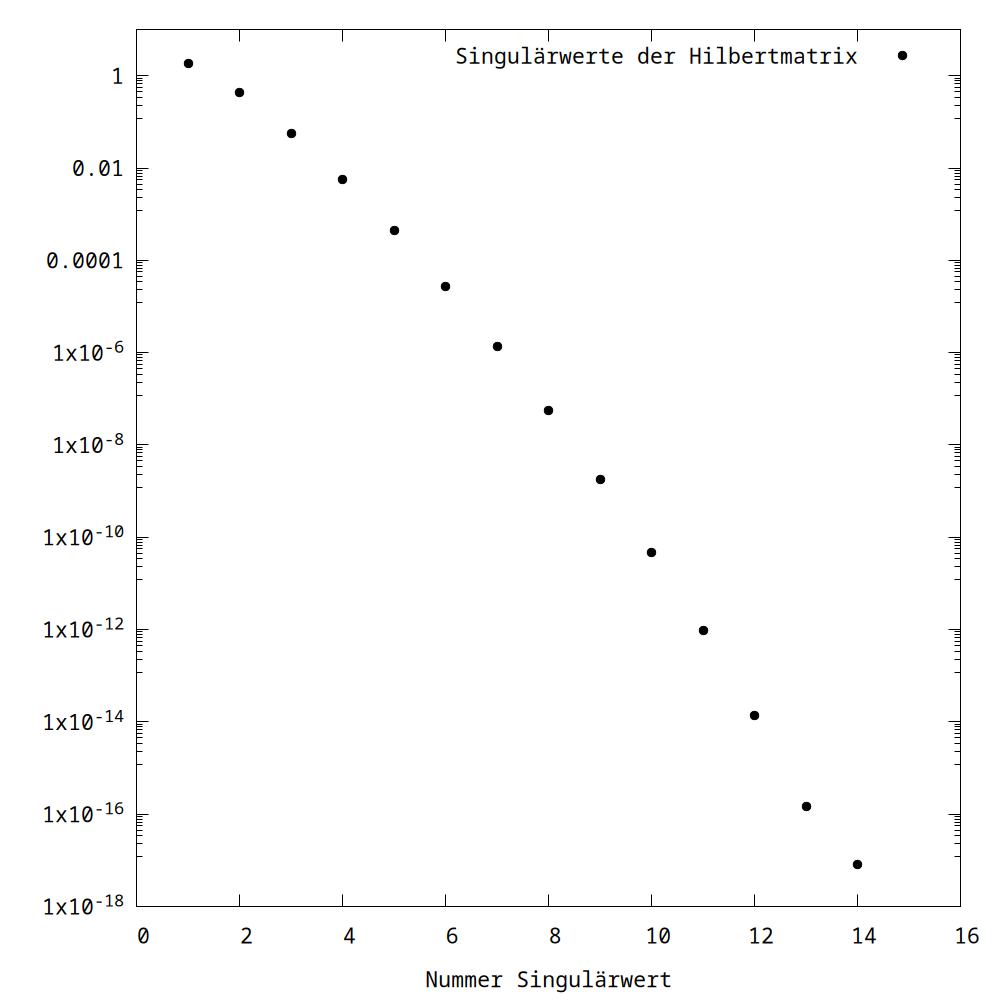
\includegraphics[width=0.45\textwidth]{./plot/hilbert15.png}}
    \qquad
    \subfloat[Fehler in $\lVert \cdot \rVert_F$ zwischen $H_n$ und bester Rang-$k$-Approximation]{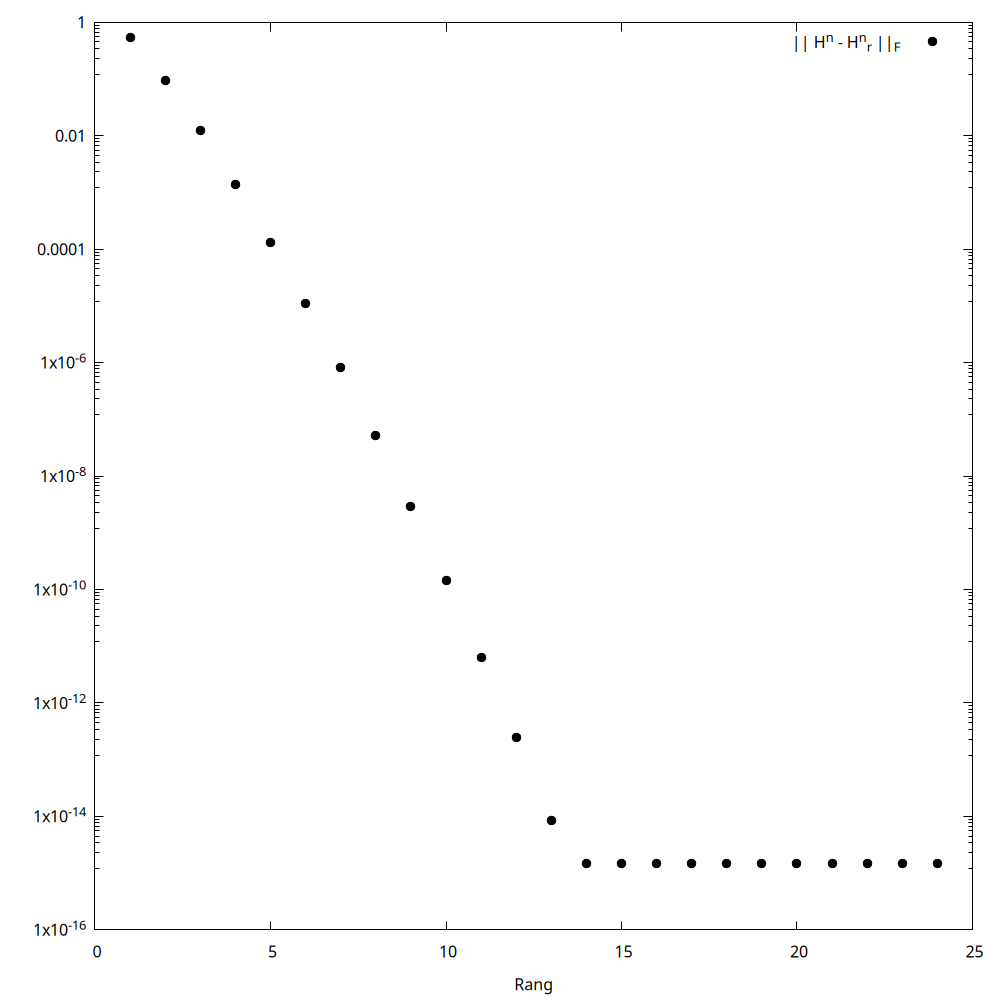
\includegraphics[width=0.45\textwidth]{./plot/errors25.png}}
\end{figure}

Die obere Abbildung zeigt die Singulärwert und Fehler bei der Rang-$k$-Approximation der Hilbertmatrix $H_n = \left(\frac{1}{i+j-1}\right)_{i=1,j=1}^{n,n}$. 
Man kann erkennen, dass die Singulärwerte sehr schnell abfallen und somit eine Approximation sehr kleinen Ranges bereits genügt, um die Matrix mit sehr kleinem Fehler darzustellen.
Ab Rang 14 gibt es keine Verbesserung mehr in der Approximation durch Erhöhen des Rangs.

\subsection{Partial Least Squares Regression (PLSR)}

Die PLSR kann man als eine Verallgemeinerung der PCA verstehen. Es werden nun zwei Datenmatritzen $X\in \R^{m \times n} ,Y \in \R^{m \times l}$ betrachtet.
Das Ziel ist eine Vorhersage der Daten von $Y$ aus den Informationen aus $X$. 
Anders als bei der PCA wird nun nicht eine Dekomposition von $X^TX$ durchgeführt, um die Varianz der Daten von $X$ zu modellieren, sondern es wird die Kovarinz
zwischen $X$ und $Y$ modelliert, in dem man die Kovarianzmatrix $X^TY$ zerlegt.

Nun wird zur Vereinfachung angenommen, dass nur eine Größe vorhergesagt werden soll.
D.h. $Y$ ist keine Matrix sondern nur ein Vektor ist $y \in \R^m$. Das Argument kann einfach auf eine Matrix erweitert werden.
Das Ziel ist eine Zerlegung von $X_k = ZV^T$, welche die beste Rang $k$-Approximation von $X$ ist, die die Kovarianz zwischen $X$ und $y$ maximiert.
Diese ist ein Vektor $\tilde{w} = ({\rm cov}(x_1,y), \cdots, {\rm cov}(x_m,y)) = (x_1^Ty, \cdots, x_m^Ty)$ mit $x_i$ sind die Zeilen von $X_k$. Es wird also die euklidische Norm dieses Vektors maximiert.
Dabei heißen die Vektoren in $Z$ PLSR-Scores und die in $V^T$ PLSR-Loadings. Und $y$ wird zerlegt in $y_k = Zb$. 
Die Approximationen von $X$ und $y$ teilen sich die Scores-Matrix. Das kann man so interpretieren, dass diese die gemeinsame Struktur der Daten modelliert.

% Source: https://allmodelsarewrong.github.io/pls.html
Der folgende Algorithmus ist iterativ. Begonnen wird mit der ursprünglichen Datenmatrix $X=:X_0$ und den vorherzusagenden Messwerten $y=:y_0$.
Die Daten sollten um den Ursprung zentriert sein. Wenn das nicht der Fall ist, kann man die selbe Methode zur Zentrierung anwenden wie bei der PCA.
Als erstes wird ein Vektor mit Kovarianzen zwischen den Spalten von $X_0$ und $y_0$ berechnet.
\begin{equation*}
    \tilde{w}_1 = (x_1^Ty, \: x_2^Ty, \: \cdots, \: x_m^Ty)
\end{equation*}

Dieser Vektor muss normiert werden:
\begin{equation*}
    w_1 = \frac{\tilde{w}_1}{\lVert \tilde{w}_1 \rVert_2}
\end{equation*}

Dann werden die Spalten von $X_0$ auf $w_1$ projeziert:
\begin{equation*}
    z_1 = \frac{X_0^Tw_1}{w_1^Tw_1}
\end{equation*}
Damit erhält man den ersten Scores-Vektor der Zerlegung der Kovarianzmatrix. 

Denn ersten Loadings-Vektor erhält man durch eine Projektion der Spalten von $X_0$ auf $z_1$:
\begin{equation*}
    v_1 = \frac{X_0^Tz_1}{z_1^Tz_1}
\end{equation*}
Die Rang-$1$-Approximation von $X$ lässt sich nun darstellen durch: $\hat{X}_1 = z_1v_1^T$.

Den ersten Regression-Parameter für $y$ erhält man durch eine Projektion von $y$ auf $z_1$:
\begin{equation*}
    b_1 = \frac{y^Tz_1}{z_1^Tz_1}
\end{equation*}
Und somit bekommt man die erste Approximation von $y$ durch: $\hat{y}_1 = b_1z_1$.

Nun berechnet man die verbleibenden Daten für den nächsten Iterationsschritt:
\begin{align*}
    X_1 = X_0 - \hat{X}_1 \\
    y_1 = y_0 - \hat{y}_1
\end{align*}

Nach $k$-Schritten erhält man so die beste Rang-$k$-Approximation von $X$ bezüglich der Kovarianz zwischen $X$ und $y$.
\cite{AMAW}

\section{MLPS}
% TODO: example pictures for erosion and dilation and opening
Der folgende Abschnitt basiert bezieht sich auf folgende wissenschaftliche Veröffentlichung: \cite{li2013morphological}
\break

Der letzte Abschnitt beschreibt eine speziellen Algorithmus zur Hintergrundkorrektur von spektralen Daten.
Spektrale Daten sind z.B. physikalische Messwerte aus einem Spektrum beispielsweise dem Lichtspektrum. 
Sie setzt sich zusammen aus Intensitäten bestimmter Wellenlängen aus dem das gemessene Signal besteht. 
Misst man beispielsweise mit einem Lichtspektrometer, welches die Intensitäten der Wellenlängen einer bestimmten Lichtquelle bestimmt, das Licht einer blauen LED,
so wird man sehen, dass hauptsächlich die Wellenlängen im Signal einen großen Einfluss haben, die blauem Licht zuzuordnen sind. Andere Wellenlängen haben keinen oder nur einen sehr geringen Einfluss.

Messungen dieser Art können durch einen Hintergrund stark verzerrt werden. In der Lichtanalogie wäre der Hintergrund zum Beispiel die Laborbeleuchtung, welche aus weißen besteht. 
Sie würde in der Messung einer bestimmten Lichtquelle alle die Intensitäten aller Wellenlängen erhöhen, sodass die Messung verfälscht wird.
Wenn der Signal-Rauschen-Abstand zu groß wird, dann ist die gesamte Messung wertlos. Deswegen muss man vor der genaueren Analyse solcher Spektraldaten den Hintergrund, welcher aus der Umgebung kommt, entfernen.

Die Arbeit beschreibt einen Algorithmus, welcher Methoden aus der mathematischen Morphologie und Penalized Least Squares verbindet.

\subsection{Mathematische Morphologie} 
Die mathematische Morphologie ist eine Technik zur Analyse geometrischer Eigenschaften.
Sie verwendet dafür topologische und megentheoretische Hilfsmittel. Zum Einsatz kommt sie hauptsächlich im Kontext der Analyse von Bildern also 2 dimensionalen Daten.
Die wissenschaftliche Arbeit hat eine Variante entwickelt, diese Technik ebenfalls auf eindimensionale Daten wie zum Beispiel spektrale Messwerte anzuwenden.

Die beiden Hauptoperationen, die in der mathematischen Morphologie genutzt werden, sind die \textbf{Dilatation} und die \textbf{Erosion} zusätzlich zu den megentheoretische Operationen (Vereinigung, Schnitt, Differenz).
Aus diesen können anschließend alle anderen Operationen zusammengestellt werden. Insbesondere die Operation der Öffnung, welche dann im MLPS-Algorithmus verwendet wird.


Bei der Beschreibung der folgenden Operationen wird eine Strukturmaske $B \subseteq \R^2$ (meistens eine Kreisfläche) verwendet und welche als Teilmenge des Bildes $A \in \R^2$ aufgefasst wird.
$B_x$ bezeichnet dann die Translation der Strukturmaske zum Punkt $x$. Dafür muss wird ein bestimmter Referenzpunkt $b \in B$ festgelegt, der nach der Translation identisch zum Punkt $x$ sein soll.
Beispielsweise könnte man für die Kreisscheibe den Mittelpunkt als Referenzpunkt wählen, sodass $B_x$ dann die Kreisscheibe mit dem Zentrum $x$ ist.

\subsubsection{Dilatation}
\begin{equation}
    {\rm Dil}(A) := \bigcup\limits_{x \in A} B_x
\end{equation}

Diese Operation transliert die Strukturmaske an jeden Punkt des Bildes $A$ und vereinigt alle Translate $B_x$. Das führt zu einem Aufblähen des Originalbilds um die Strukturmaske.

\subsubsection{Erosion}
\begin{equation}
    {\rm Er}(A) := \bigcup \{B_x \: | \: x \in A \land B_x \subseteq A\}
\end{equation}

Diese Operation transliert die Strukturmaske ebenfalls an jeden Punkt des Bildes, vereinigt jedoch nur die Translate, welche sich vollständig im Ursprünglichen Bild befinden.
Das führt zu einer Verkleinerung des Bildes. Lange dünne Spitzen, die aus dem Bild herausragen, werden je nach Größe und Form der Strukturmaske abgeschnitten.

\subsubsection{Öffnung}

Die Öffnung ist die Hintereinanderausführung von Erosion und Dilatation, also:
\begin{equation}
    {\rm Op}(A) := ({\rm Dil} \circ {\rm Er})(A) = {\rm Dil}({\rm Er}(A))
\end{equation}

Wie beschrieben entfernt die Erosion Spitzen, die aus dem Bild herausragen und die anschließende Dilatation macht die Errosion an dem verbleibenden Stellen wieder rückgängig.
\cite[Kapitel 12]{sichtprufungautomatische}

\subsubsection{Im Kontext von MLPS}

Nun wird nicht mehr mit 2 dimensionalen Bildern als Eingabe gearbeitet sondern mit eindimensionalen Messwerten. Die Daten werden in einem $(x,y)$-Koordinatensystem abgetragen. 
Sei nun $(x,f(x)) \in \R^2$ ein Messwert. Somit sei $f:\R \to \R$ die Funktion, die für alle $x \in \R$ den gemessenen Wert ausgibt. Als eindimensionales Analogon zur Kreisscheibe wird nun ein Intervall verwendet. 
Dieses Fenster sei $W_x := [x-w, x+w]$ mit $w \in \R_+$. Die halbe Fensterbreite $w$ ist dabei ein Hyperparameter, der manuell festgelegt werden muss. 
Dieses Fenster wird nun so transliert, dass sein Zentrum mit $x$ übereinstimmt.

Für die Dilatation wird dann das Maximum über die im Fenster befindlichen Messwerte genommen und für die Erosion jeweils das Minimum. Somit gilt:

\begin{align}
    {\rm Er}(x)  &= \min\limits_{\tilde{x} \in W_x} f(\tilde{x}) \\
    {\rm Dil}(x) &= \max\limits_{\tilde{x} \in W_x} f(\tilde{x})
\end{align}

Die Definition def Öffnung bleibt gleich, wie im 2 dimensionalen Fall.
Für echte Daten muss dieses Definition noch diskretisiert werden, weil die Messwerte nicht durch eine Funktion $f$ die auf ganz $\R$ existiert, definiert sind, sondern eine diskrete Menge von Punkten $X := \{(x_i,y_i) \in \R^2 \: | \: n\in \mathbb{N}, i=1,\cdots,n \}$.

Die beiden Operatoren ändern sich für jedes $i\in \{1,\cdots,n\}$ zu:
\begin{align}
    {\rm Er}(x_i) &= \min \{y_{i+j} \: | \: j=-w,\cdots,w \: \land \: 0 \leq i + j \leq n\} \\
    {\rm Dil}(x_i)  &= \max \{y_{i+j} \: | \: j=-w,\cdots,w \: \land \: 0 \leq i + j \leq n\}
\end{align}

Dabei ist $w \in \mathbb{N}$ nun eine diskrete Fenstergröße.

\subsection{Penalized Least Squares}
Penalized Least Square ist eine Variante der Least Squares Optimierung.

\subsubsection{Least Squares}
Seien folgende Gleichungen gegeben:
\begin{align}
    Ax = b \label{eq:ls} \\ 
    \min\limits_{x \in \R^n} \lVert b - Ax \rVert \label{eq:minls}
\end{align}
$x \in \R^n, b \in \R^m, A \in \R^{m\times n}$.

Das gewöhnliche Least-Squares-Verfahren wird verwendet, um ein lineares Gleichugssystem zu lösen. 
Dieses kann als Matrix-Vektor-Produkt dargestellt werden wie in Gleichung \ref{eq:ls}. 
Aus dieser kann man das Minimierungsproblem herleiten wie in Gleichung \ref{eq:minls}.

Wenn $A$ nicht invertierbar ist und $b$ nicht im Spaltenraum von $A$ liegt, dann existiert keine Lösung für Gleichung \ref{eq:ls}.
Das Minimierungsproblem \ref{eq:minls} liefert dann eine beste Approximation der Lösung der Gleichung. 
Diese Approximation muss aber nicht notwendig eindeutig bestimmt sein. 
Denn angenommen $\hat{x}$ löst das Minimierungsproblem \ref{eq:minls}, dann gilt für $\forall y \in \mathcal{N}(A)$:
\begin{equation}
    \min\limits_{x \in \R^n} \lVert b - A(\hat{x} + y) \rVert = \min\limits_{x \in \R^n} \lVert b - A\hat{x} - Ay \rVert = \min\limits_{x \in \R^n} \lVert b - A\hat{x} \rVert
\end{equation}

Um dieses Problem zu vermeiden, wird der Nullraum von $A$ verworfen. 
Man erhält eine Abbildung $f: \mathcal{N}(A)^{\bot} \to R(A)$.

\begin{lemma}\label{lem:fbij}
    Die Abbildung $f: \mathcal{N}(A)^{\bot} \to R(A),\: x \mapsto Ax$ ist bijektiv und linear.
\end{lemma}

\begin{proof}
    Die Linearität von $f$ folgt direkt aus der Definition von $f$.

    \textit{Surjektivität}: Sei $y \in R(A)$. Das heißt es existiert ein Element $x \in \R^n$, sodass $Ax = y$. 
    
    Aus $\R^n = \mathcal{N}(A) \oplus \mathcal{N}(A)^{\bot}$ folgt, dass es $x_1 \in \mathcal{N}(A), x_2 = \mathcal{N}(A)^{\bot}$ mit $x = x_1 + x_2$.

    \begin{equation}
        y = Ax = A(x_1 + x_2) = Ax_1 + Ax_2 = Ax_2
    \end{equation}
    Also $Ax_2 = f(x_2) = y$ mit $x_2 \in \mathcal{N}(A)^{\bot}$.

    \textit{Injektivität}: Seien $x_1, x_2 \in \mathcal{N}(A)^{\bot}$ mit $f(x_1) = f(x_2) = y \in R(A)$. Daraus folgt, dass $Ax_1 - Ax_2 = A(x_1 - x_2) = 0$ und somit $x_1 - x_2 \in \mathcal{N}(A)$.
    
    Nach Wahl von $x_1$ und $x_2$ folgt: $x_1 - x_2 \in \mathcal{N}(A)^{\bot} \cap \mathcal{N}(A) = \{0\} \Rightarrow x_1 = x_2$.

\end{proof}

Nach Lemma \ref{lem:fbij} existiert eine eindeutig bestimmte Inverse $f^{-1}: R(A) \to \mathcal{N}(A)^{\bot}$. Das rechtfertigt nun folgende Definition:
\begin{defin}\label{defin:pinv}
    Sei $A \in \R^{m \times n}$. Die \textbf{Moore-Penrose-Pseudoinverse} $A^{\dagger}$ (aufgefasst als Abbildung $x \mapsto A^{\dagger}x$) der Matrix $A$ 
    ist definiert als die eindeutig bestimmte lineare Fortsetzung von $f^{-1}: R(A) \to \mathcal{N}(A)^{\bot}$ mit ${\rm Ker}A^{\dagger} = R(A)^{\bot}$.
    Dabei ist $f$ wie oben definiert also $f: \mathcal{N}(A)^{\bot} \to R(A),\: x \mapsto Ax$.
\end{defin}

\begin{lemma}\label{lem:pinvp}
    Für $A \in \R^{m \times n}$ gilt: $A^{\dagger}A = P_{\mathcal{N}(A)^{\bot}}, \: AA^{\dagger} = P_{R(A)}$, wobei $P_X$ der orthogonale Projektor auf den Unterraum $X$ ist.
\end{lemma}

\begin{proof}\cite[S. 255, Satz 4.8.5.1]{stoer2005numerisch}
    Sei $f^{-1}: R(A) \to \mathcal{N}(A)^{\bot}$ die Abbildung aus Definition \ref{defin:pinv}. Sei $x \in R^{m} = R(A) \oplus R(A)^{\bot}$, 
    also existieren $x_1 \in R(A), x_2 \in R(A)^{\bot}$ mit $x = x_1 + x_2$. Nach Definition von $A^{\dagger}$ folgt:
    \begin{equation}
        A^{\dagger}x = A^{\dagger}(x_1 + x_2) = A^{\dagger}x_1 + A^{\dagger}x_2 = A^{\dagger}x_1 = f^{-1}(x_1)
    \end{equation}
    
    Somit gilt die Gleichung für $\forall x \in \R^n$:
    \begin{equation}
        A^{\dagger}x = (f^{-1} \circ P_{R(A)})(x)
    \end{equation}
    und damit folgt:
    \begin{equation}
        A^{\dagger}Ax = f^{-1}(P_{R(A)}(Ax)) = f^{-1}(Ax) = P_{\mathcal{N}(A)^{\bot}}x
    \end{equation}

    Nun sei $y \in \R^m$:
    \begin{equation}
        AA^{\dagger}y = A(f^{-1}(P_{R(A)}x)) = P_{R(A)}y
    \end{equation}
\end{proof}

\begin{thm}\label{thm:pinvu}
    Sei $A \in \R^{m \times n}$ und $y \in \R^m$. Dann gilt für $\hat{x} = A^{\dagger}y$:
    \begin{enumerate}
        \item $\lVert Ax - y \rVert_2 \geq \lVert A\hat{x} - y \rVert_2$ für $\forall x \in \R^m$,
        \item Sei $x \in \R^n$: $\lVert Ax - y \rVert_2 = \lVert A\hat{x} - y \rVert_2 \Rightarrow \lVert x \rVert_2 > \lVert \hat{x} \rVert_2$
    \end{enumerate}
\end{thm}

\begin{proof}\cite[S. 256, Satz 4.8.5.4]{stoer2005numerisch}
    
    Beweis von 1.:
    
    Sei $y \in R^m$ und $\hat{x} = A^{\dagger}y$. Nach Lemma \ref{lem:pinvp} gilt $AA^{\dagger} = P_{R(A)}$. Somit gilt für $\forall x \in \R^n$:
    \begin{align}
        &Ax - y = u - v \\
        &u := A(x - A^{\dagger}y) \in R(A), \: v:=(I-AA^{\dagger}) = y - A\hat{x} \in R(A)^{\bot}
    \end{align}
    Es folgt:
    \begin{equation}
        \lVert Ax - y \rVert^2_2 = \lVert u \rVert^2_2 + \lVert v \rVert^2_2 \geq \lVert v \rVert^2_2 = \lVert A\hat{x} - y\rVert^2_2
    \end{equation}
    Gleichheit gilt, genau dann wenn $u = 0$, also $Ax = AA^{\dagger}y$.

    Beweis von 2.:

    Nach Lemma \ref{lem:pinvp} gilt auch noch, dass $A^{\dagger}A = P_{\mathcal{N}(A)^{\bot}}$. Es gilt für alle $\forall x \in \R^n$ 
    mit $Ax = AA^{\dagger}y$:
    \begin{align}
        &x = u_1 + v_1 \\
        &u_1 := A^{\dagger}A x = A^{\dagger}AA^{\dagger}y = A^{\dagger}y = \hat{x} \in \mathcal{N}(A)^{\bot} \\
        &v_1 := x - u_1 = x - \hat{x} \in \mathcal{N}(A)
    \end{align}
    und damit $\lVert x \rVert^2_2 > \lVert \hat{x} \rVert^2_2$ für $\forall x \in \R^n: x \neq \hat{x}$ mit $\lVert Ax - y \rVert_2 = \lVert A\hat{x} - y\rVert_2$.


\end{proof}

Durch Satz \ref{thm:pinvu} kann man nun die Lösung des Least Squares Optimierungsproblems darstellen mithilfe der Pseudoinversen, also $\hat{x} = A^{\dagger} b$.
Diese ist die eindeutig bestimmte Lösung, die \ref{eq:minls} erfüllt und von allen Lösungen, die ebenfalls \ref{eq:minls} erfüllen, besitzt $\hat{x}$ die kleinste Norm.

\subsubsection{Penalized Least Squares als Erweiterung von Least Squares}
Penalized-Least-Squares erweitert das Optimierungsproblem aus \ref{eq:minls} nun um ein Regularisierungsfunktional der Form $R: \R^n \to \R$.
Die neue Optimierungsproblem hat dann die Form:

\begin{equation}
    \min\limits_{x \in \R^n} \lVert b - Ax \rVert + \lambda R(x)
\end{equation}
wobei $\lambda \in \R$ wieder ein Hyperparameter ist, welcher den Einfluss der Regularisierungen steuert.

Spezielle zu erwähnen sind die LASSO und $\ell^2$-Regularisierungen. Für LASSO gilt: $R: \R^n \ni x \mapsto \lVert x \rVert_1$ und für die $\ell^2$-Regularisierung gilt: $R: \R^n \ni x \mapsto \lVert x \rVert_2$.
LASSO liefert dabei dünnbesetzte Lösungen mit vielen Nulleinträgen. 
$\ell^2$ hält die Norm der Lösung beschränkt, sodass es keine besonders großen Werte in $\hat{x}$ gibt.

\cite[S. 184f.]{strang2019linear}

\subsection{Signal Hintergrundkorrektur}

Im folgenden Abschnitt gilt: $x \in \R^n$ ist der Vektor der Messwerte eines Signals. 

Als erstes führt der Algorithmus eine diskrete morphologische Öffnung mit den Messwerten $x$ durch. Dabei muss eine Fenstergröße $w$ für den Algorithmus festgelegt werden.
In der wissenschaftlichen Arbeit wurde mit den verschiedenen Fenstergrößen ($w=11,13,15$) experiementiert, welche alle zu einem sehr ähnlichen Ergebnis führten.
Die Öffnung bringt nun eine grobe erste Schätzung für das Hintergrundspektrum, welches entfernt werden soll.
An den Peaks der Messung kann man jedoch erkenne, dass sich durch die Öffnung Plateaus formen, sodass das Hintergrundspektrum dort nur sehr schlecht approximiert ist.

Um diesen Effekt zu mindern, wird nun PLSR zusätzlich angewandt.

Als Regularisierungsfunktional nutzt MLPS die Rauhigkeit der Least-Squares-Lösung.
\begin{equation}
    R: \R^n \ni x \mapsto \sum_{i=2}^{n} (x_i - x_{i-1})^2 = \lVert Dx \rVert_2
\end{equation}
wobei $D \in \R^{n\times n}$ definiert ist durch $(d_{ij})_{i=1,j=1}^{n-1,n} = (\delta_{i,j-1} - \delta_{i,j})_{i=1,j=1}^{n-1,n}$ ($\delta_{i,j}$ ist das Kronecker-Delta).

Ohne die morphologische Analyse wäre das PLSR-Minimierungsproblem folgendes:
\begin{equation}\label{eq:plsreq}
    \min\limits_{z \in \R^n} F + \lambda R = \min\limits_{z \in \R^n} \lVert x - z \rVert_2^2 + \lambda \lVert Dz \rVert_2    
\end{equation}
wobei $\lambda \in R_{\geq0}$ ein Hyperparameter ist, denn man wählen. Umso größer man ihn wählt, umso glatter wird die Lösung.
$F$ ist dabei die Summe der quadratischen Abstände zwischen $x$ und $z$.

Nun wird zusätzlich die Information der morphologischen Öffnung eingebracht.
Man bestimmt die Minima zwischen den Plateaus, die durch die Öffnung der analytischen Daten entstehen. 
Als erstes werden die Start- und Endpunkte dieser Plateaus bei den Peaks bestimmt.
Sei $s_k \in \N$ der Index des Startpunkts und $e_k \in \N$ der Index des Endpunktes des Plateaus am $k$-ten Peaks. Das $k$-te Minimum ist nun definiert durch:
\begin{equation}
    M_k = \arg\min \{x_j \: | \: j=e_k,\cdots s_{k+1}\}
\end{equation}
Sei $M := \{M_k \: | \: k \in \{0, \cdots, p\}\}$, wobei $p \in \mathbb{N}$ die Anzahl der Peaks in den Daten $x$ angibt.

Nun erstellt man einen Vektor mit Gewichten $w \in \R^n$. Die $i$-te Stelle des Vektors sei $w_i$. Dann ist dieser Vektor wie folgt definiert:
\begin{equation}
    w_i = \begin{cases}
        1, \: i \in M, \\
        \varepsilon, \: i \notin M.
    \end{cases}
\end{equation} 
mit $\varepsilon \in [0, 1)$ klein gewählt, z.B. $\varepsilon = 0$.

Man gewichtet nun die Summe der qudratischen Differenzen mit einer Matrix $W := (\delta_{ij} w_i)_{i=1, j=1}^{m,m}$. Also ist $F$ nun:
\begin{equation}\label{eq:Fmod}
    F = \sum\limits_{i=1}^m (x-z)^TW(x-z)
\end{equation}
Diese Gewichtung bevorzugt die Stellen, an denen ein lokales Minimum vorherrscht und korregiert somit die Plateaus, die über das Spektrum hinausragen, nach unten.

Wenn man nun in das Optimierungsproblem aus Gleichung \ref{eq:plsreq} die gewichtete Version von $F$ aus Gleichung \ref{eq:Fmod} einsetzt und das Problem löst, erhält man folgenden Lösungsvektor:
\begin{equation}
    z = (W + \lambda D^TD)^{-1}Wx
\end{equation}

Die Lösung $z$ ist nun das ein glattes, approximierte Hintergrundspektrum der Daten in $x$.
Man kann erkennen, dass nach der Regression die Plateaus verschwunden sind und der Hintergrund besser approximiert wird als durch die isolierte Anwendung der morphologischen Methoden. 

\clearpage
\bibliographystyle{alpha}
\bibliography{ref} % see references.bib for bibliography management

\end{document}